\documentclass[12pt]{article}

% This first part of the file is called the PREAMBLE. It includes
% customizations and command definitions. The preamble is everything
% between \documentclass and \begin{document}.

\usepackage[margin=1in]{geometry}  % set the margins to 1in on all sides
\usepackage{graphicx}              % to include figures
\usepackage{amsmath}               % great math stuff
\usepackage{amsfonts}              % for blackboard bold, etc
\usepackage{amsthm}                % better theorem environments
\usepackage{amssymb} 
\usepackage{mathptmx}
\usepackage{enumerate}
\usepackage{listings}
\usepackage{xcolor}
\usepackage{forest}
\usepackage{tabularx}  

% various theorems, numbered by section

\newtheorem{thm}{Theorem}[section]
\newtheorem{lem}[thm]{Lemma}
\newtheorem{prop}[thm]{Proposition}
\newtheorem{cor}[thm]{Corollary}
\newtheorem{conj}[thm]{Conjecture}
\newtheorem{mydef}[thm]{Definition}
\lstset{
	basicstyle          =   \sffamily,          
	keywordstyle        =   \bfseries,          
	commentstyle        =   \rmfamily\itshape,  
	stringstyle         =   \ttfamily,  
	flexiblecolumns,                
	numbers             =   left,   
	showspaces          =   false,  
	numberstyle         =   \fontsize{5}{skip},    
	showstringspaces    =   false,
	captionpos          =   t,      
	frame               =   lrtb,   
}

\lstdefinestyle{cpp}{
	language        =   cpp, 
	basicstyle      =   \fontsize{5}{skip},
	numberstyle     =   \fontsize{5}{skip},
	keywordstyle    =   \color{blue},
	keywordstyle    =   [2] \color{teal},
	stringstyle     =   \color{magenta},
	commentstyle    =   \color{red}\ttfamily,
	breaklines      =   true,   
	columns         =   fixed,  
	basewidth       =   0.5em,
}
\begin{document}


\title{ CSE 102 Spring 2021\\
	Homework Assignment 5}

\author{Jaden Liu \\ 
University of California at Santa Cruz\\
Santa Cruz, CA 95064 USA }

\maketitle


\section{HW5} 
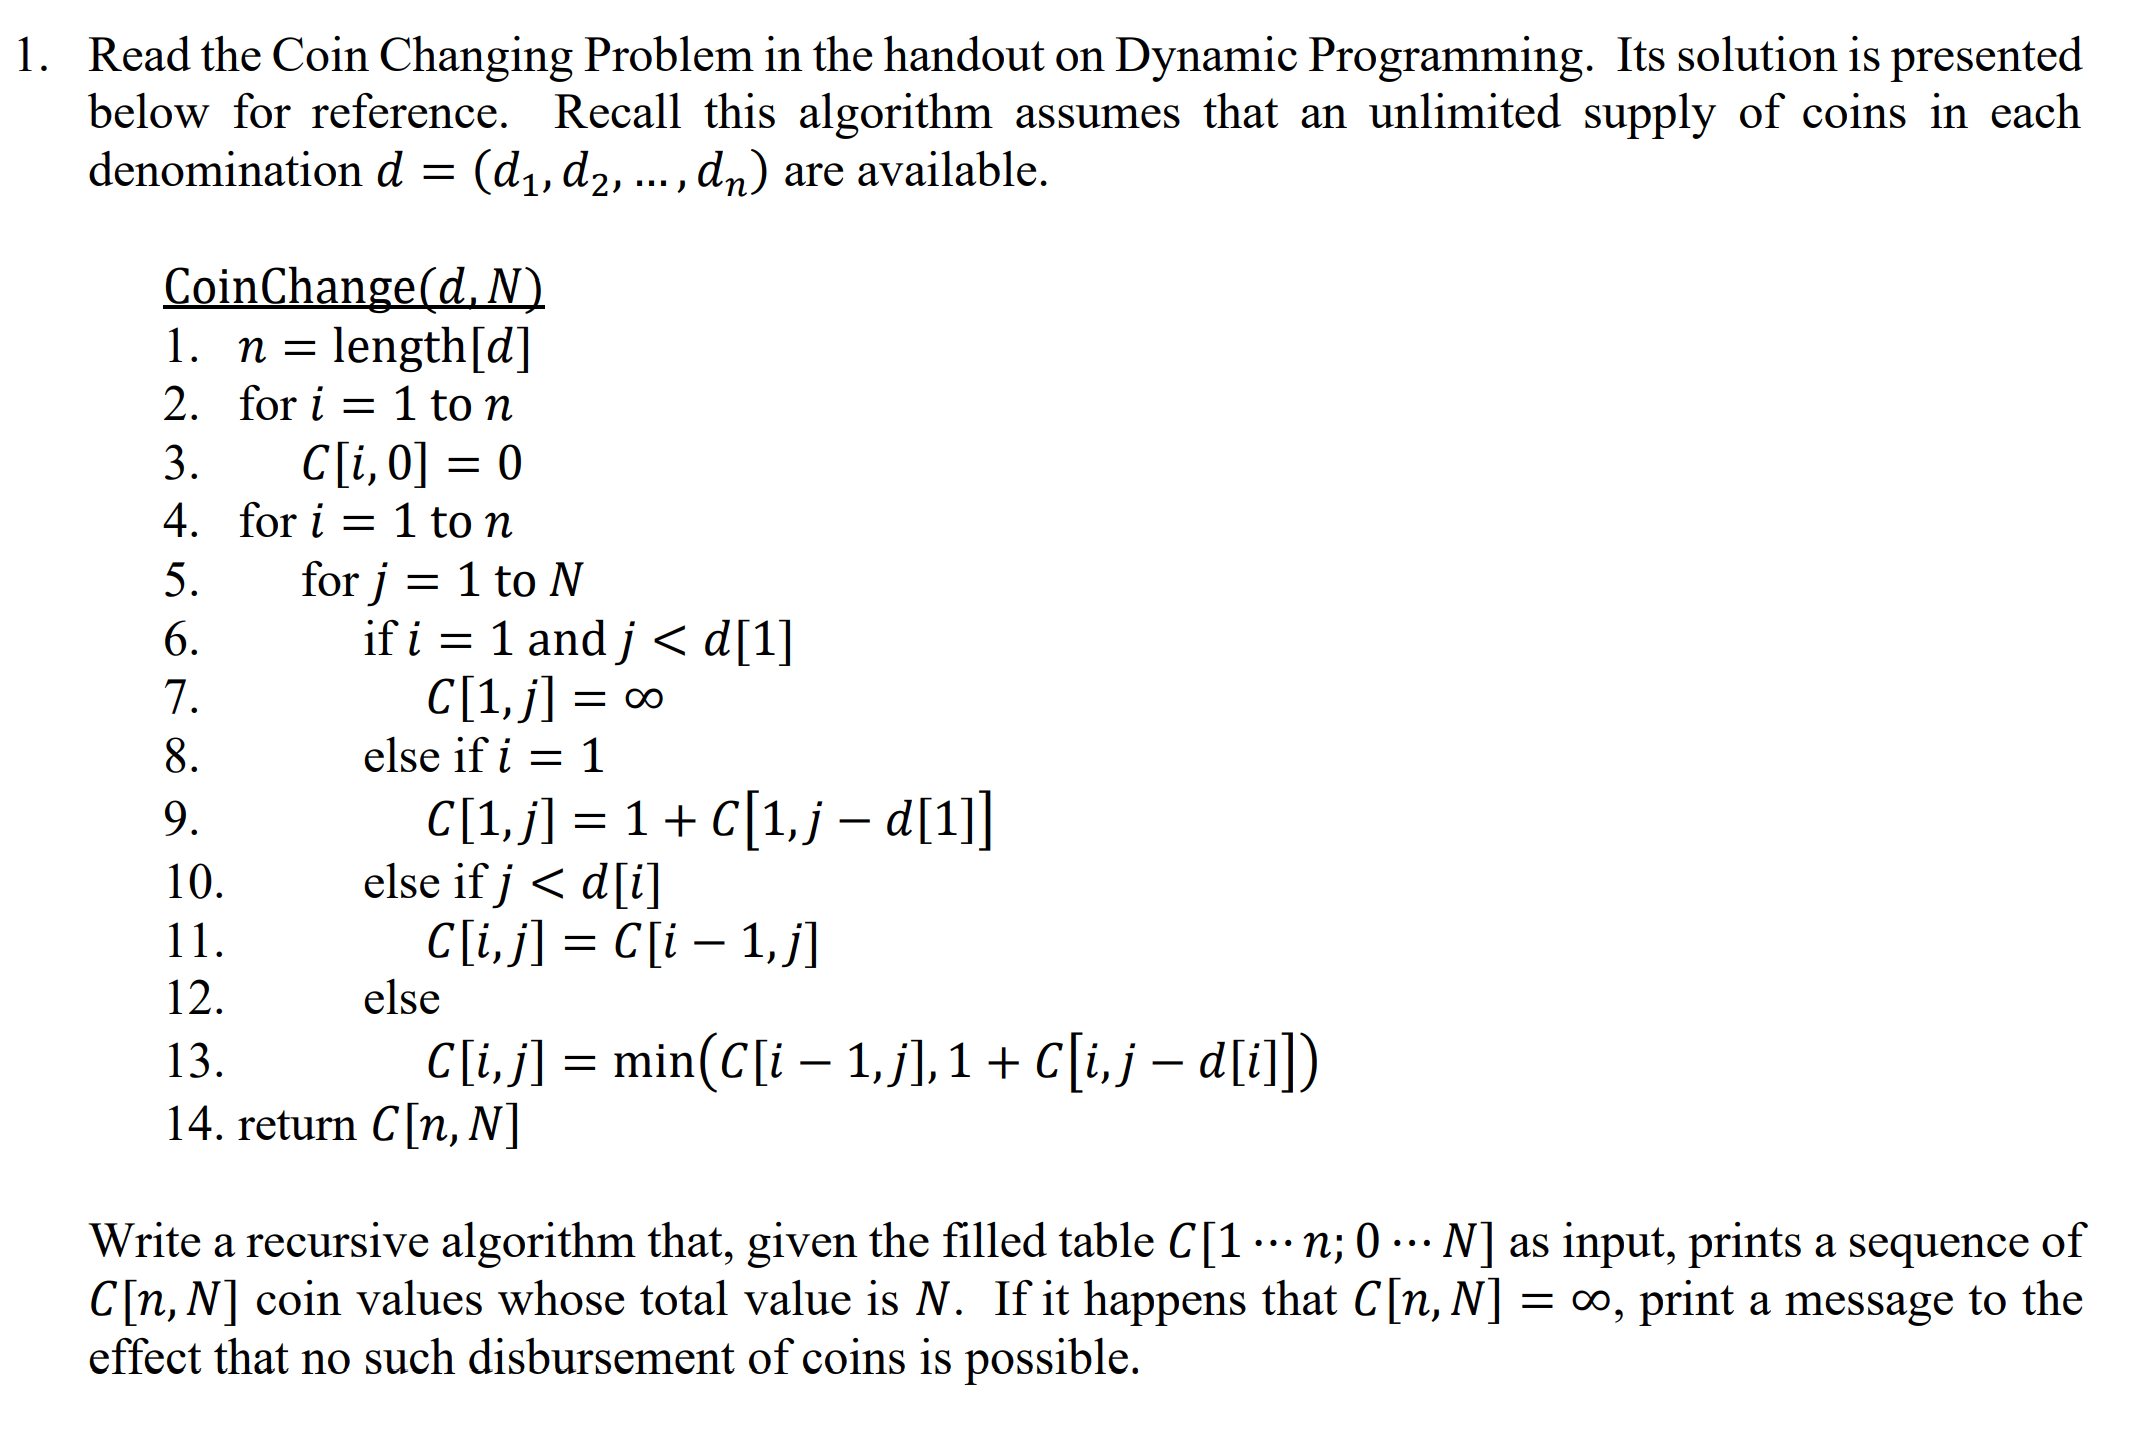
\includegraphics[scale=0.22]{1.png}
\begin{proof}[Solution]
	Since  C[i][j] will always comes from C[i-1][j] or C[i][j-d[i]], so we just need to recursively see back the process then we will find all sequence of C[n,N].\\
	
	If C[i][j] = C[i-1][j], it means that we didn't increase any more coin, so we don't need to print the coin now
	
	If C[i][j] =C[i][j-d[i]], it means that we find a better solution by adding the present coin, so we need to print it out.
	
	Keep finding until we reach the end of the table.\\
	Here is pseudo code:\\
	\begin{lstlisting}[language={python},numbers=left,numberstyle=\tiny,%frame=shadowbox,  
		rulesepcolor=\color{red!20!green!20!blue!20},  
		keywordstyle=\color{blue!70!black},  
		commentstyle=\color{blue!90!},  
		basicstyle=\ttfamily]  
		
coin(C[][], n,N)
	if C[n][N] == $\infty$
		print("no such disbursement")
	if n<=0 or N<=0
		return
	if C[n][N] == C[n][N-d[n]]:
		print d[n]
		coin(C[][], n, N-d[n])
	else:
		coin(C[][], n-1, N)
	\end{lstlisting}
\end{proof}
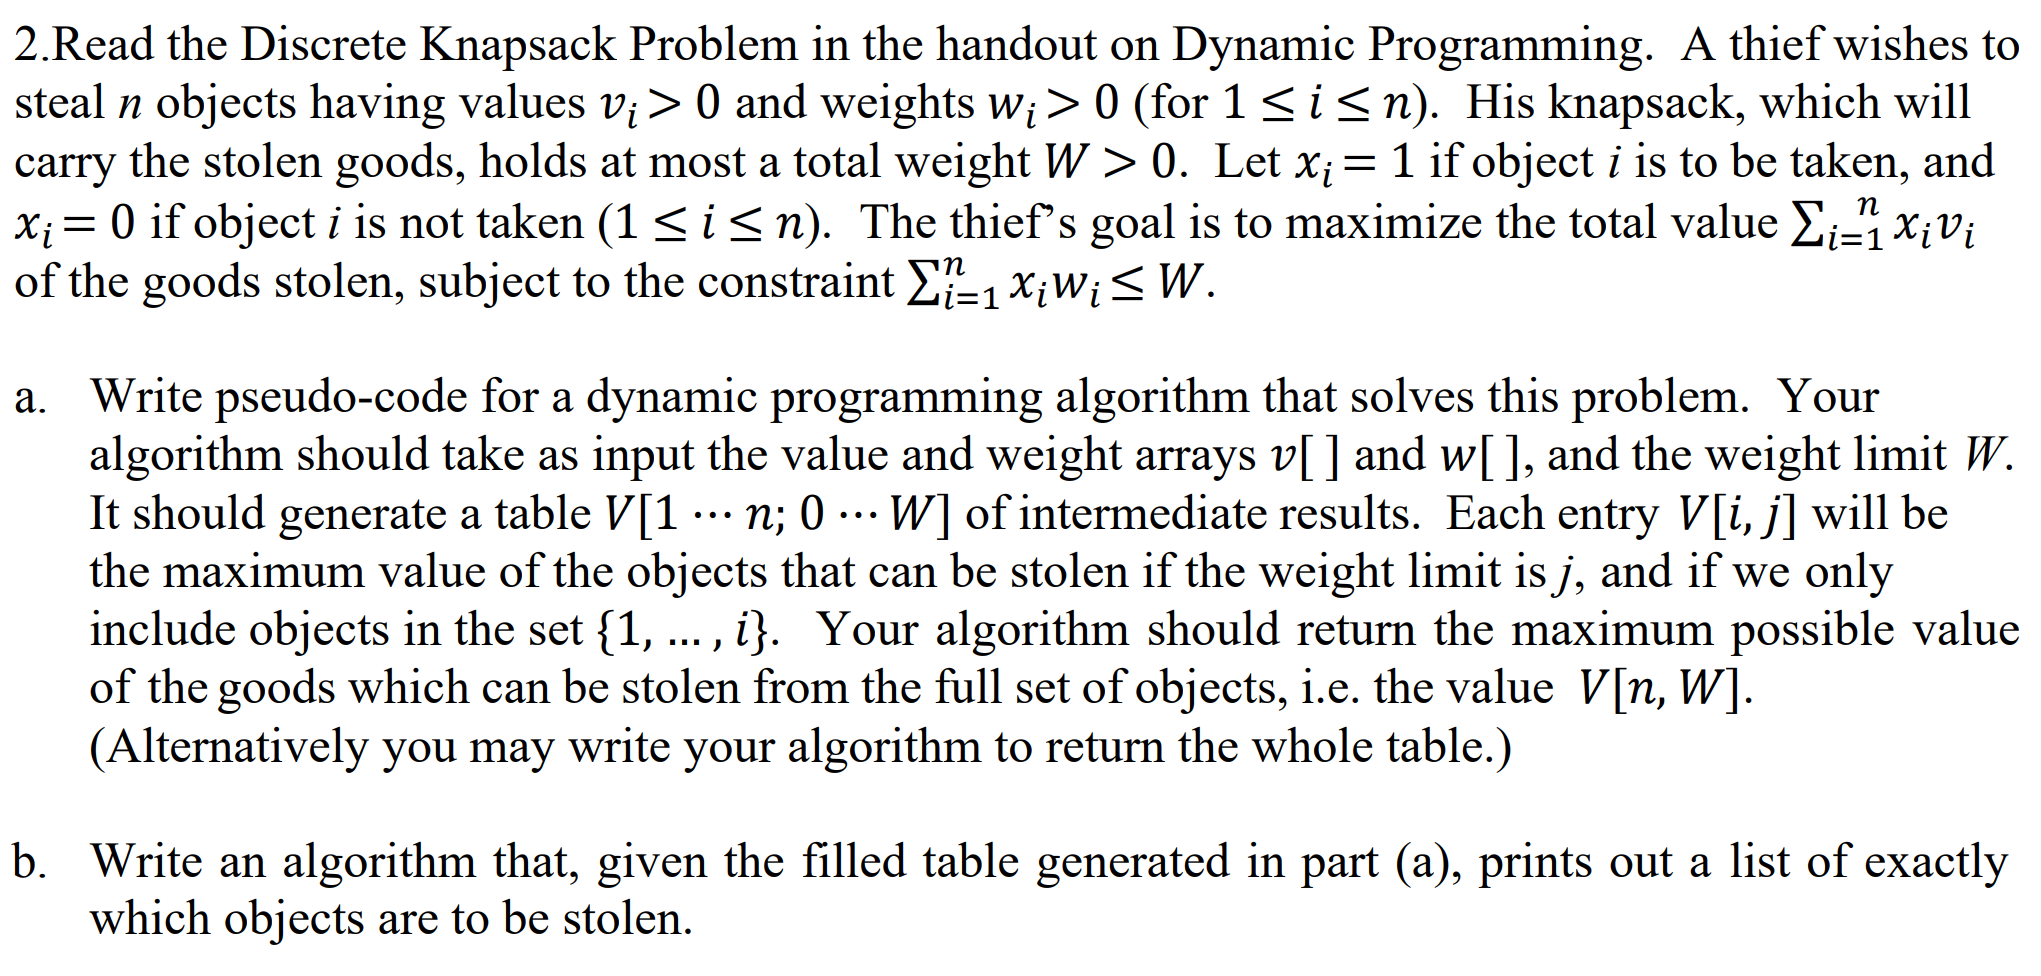
\includegraphics[scale=0.22]{2.png}
\begin{proof}[Solution for a]
	\ \\
	\begin{lstlisting}[language={python},numbers=left,numberstyle=\tiny,%frame=shadowbox,  
		rulesepcolor=\color{red!20!green!20!blue!20},  
		keywordstyle=\color{blue!70!black},  
		commentstyle=\color{blue!90!},  
		basicstyle=\ttfamily]  
		
knapsack(v[],w[],w,n)
	V[][] = int[w+1][v+1]
	for i=1 to n:
		for j=1 to w:
			if j>w[i]:
				V[i][j] = max(V[i-1][j],V[i-1][j-w[i]]+v[i])
			else:
				V[i][j] = V[i-1][j]
	return V[n][w]
	\end{lstlisting}
\end{proof}
\begin{proof}[Solution for b]
	The solution is similar to question 1. Since all V[i][j] comes from either V[i-1][j] or V[i-1][j-[wi]]+v[i]. Then we only needs to compare V[i][j] with these two values and we will get the souce of the value, or the objects to stolen.
	
	If V[i][j] = V[i-1][j], that means we cannot put it in the bag in the subproblem. Thus, we don't need to save the object.
	
	If V[i][j] = V[i-1][j-[wi]]+v[i], which means we have put the object i into our bag, save the value.
	
	Keep recursively find in either V[i-1][j], or V[i-1][j-[wi]]+v[i] in the situation above until we reach the end of the table.
\end{proof}
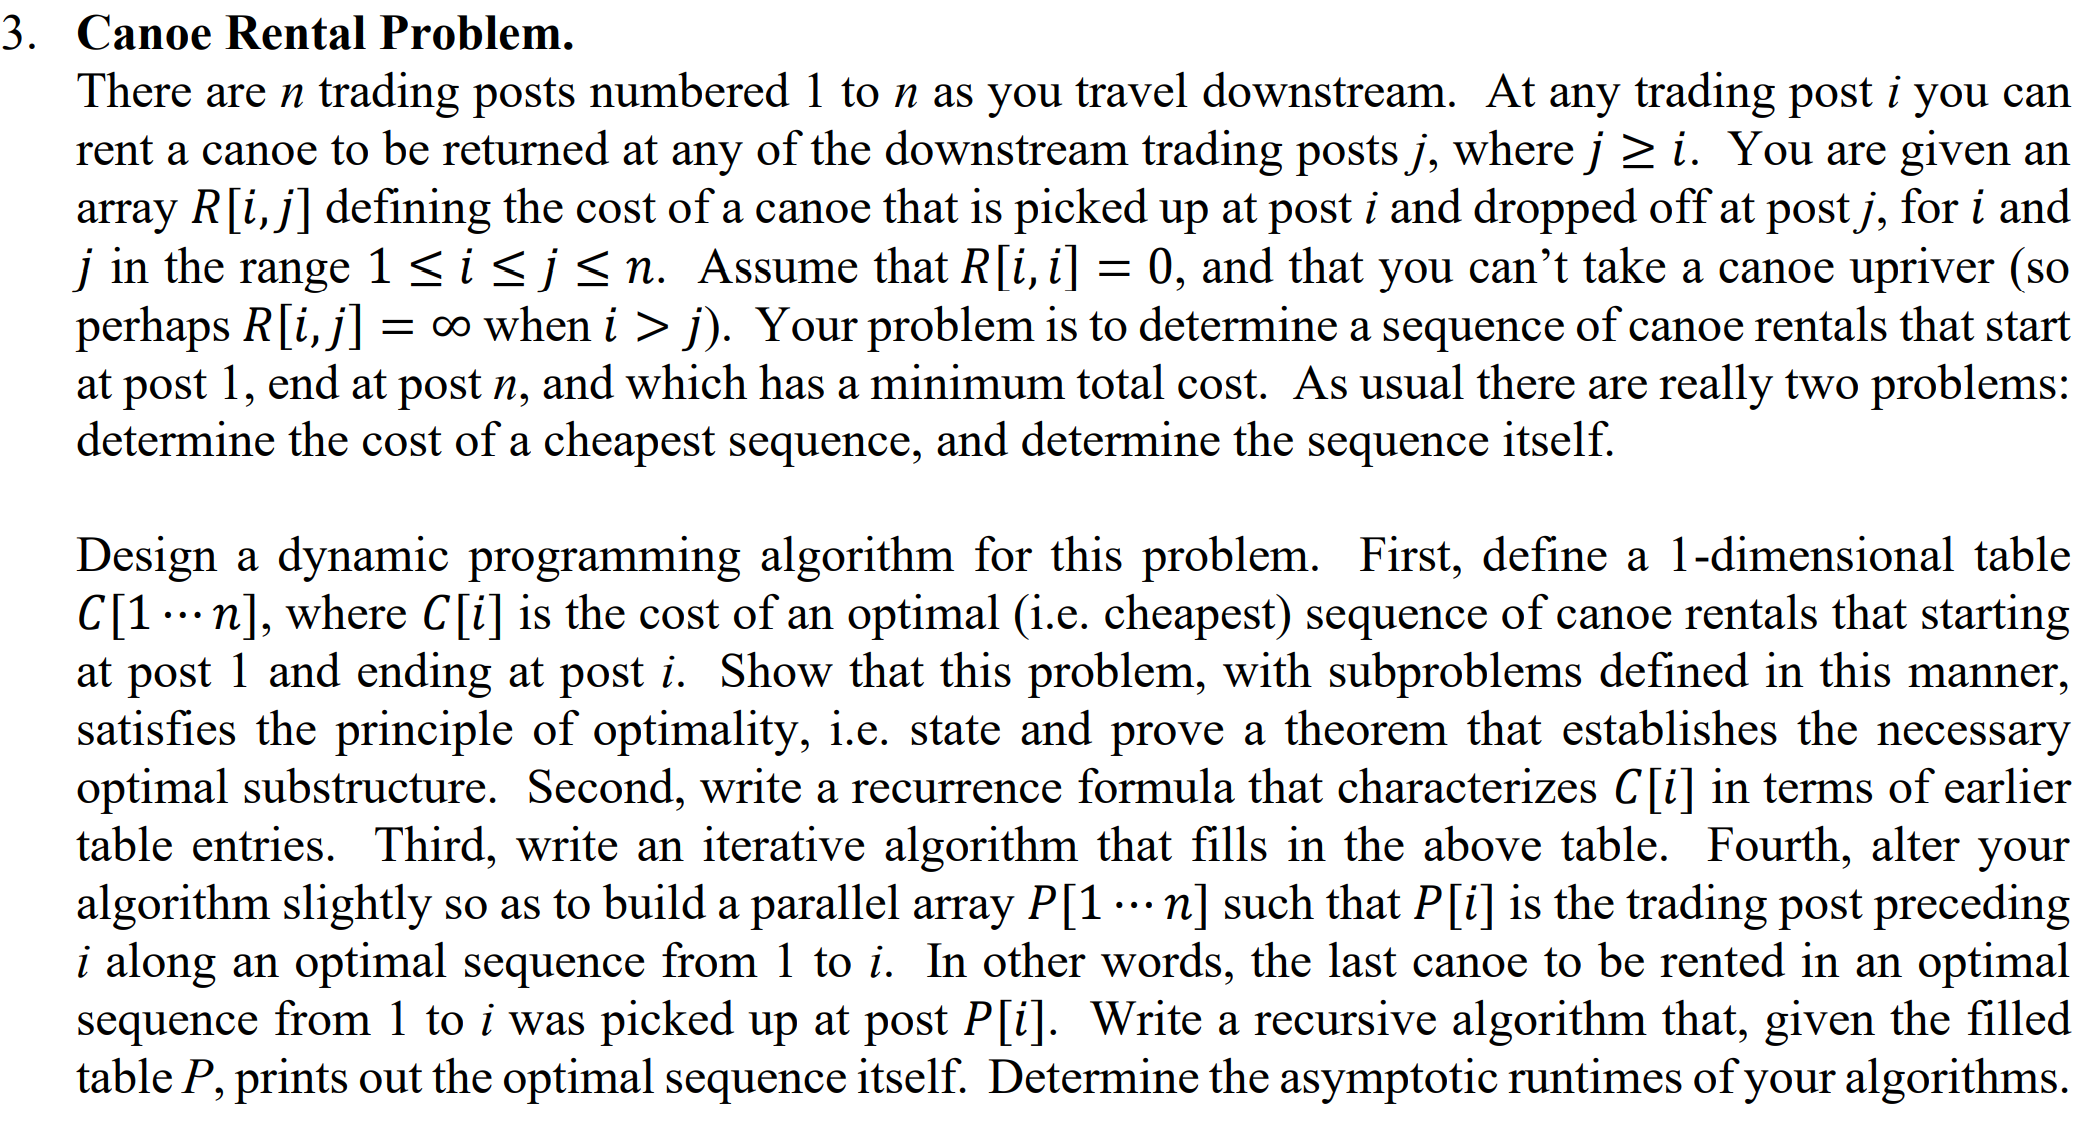
\includegraphics[scale=0.22]{3.png}
\begin{proof}[Proof for 3.1]
	Let P to be the optimal soltuion for $C[i]$, and let P' to be the subsequence of P = R(k,i)+C[k] in the path P. Assume, to the contradiction, that P' is not the optimal. Then there exist a P''=R(s,i)+C[s]. Then we can replace P' with P'' to obtain a shorter path than P. This contradicts that P is the shortest path in the initial. Therefore, it satisfy the principle of optimality.
\end{proof}
\begin{proof}[Recurrence]
	$C[i] = min(R(k,i)+C[k])$, $1<k<n$, so that k is the optimal minimum cost that makes R(k,i) + C[k] least.
\end{proof}
\begin{proof}[Algorithm]
	\begin{lstlisting}[language={python},numbers=left,numberstyle=\tiny,%frame=shadowbox,  
		rulesepcolor=\color{red!20!green!20!blue!20},  
		keywordstyle=\color{blue!70!black},  
		commentstyle=\color{blue!90!},  
		basicstyle=\ttfamily]  
		
fill(C[],i):
	for j=1 to i:
		if j<=1:
			return 0;
		min = $\infty$;
		for l=1 to j:
			temp = R(l,i)+C[i]
			if temp < min:
				min = temp
		C[j] = min
	return c[]
	\end{lstlisting}
\end{proof}
\begin{proof}[Parellel array]
	Adding a flag to denote the k in step min(R(k,i)+C[k]), and saving it into P[i].\\
	Since P[i] was saved the last post, so we continue find in P[P[i]] until we reach the first post.\\
	The time to find single C[i] is O(n), the outer loop that find C[i] to C[n] also needs O(n), therefore, the runtimes for determining the cost of a cheapset seqeuence is $O(n^2)$.\\
	While for the algorithm that determines the sequence, it cost O(n) in the worst case. O(1) in the best case, depending on the array P.
\end{proof}
\bigskip
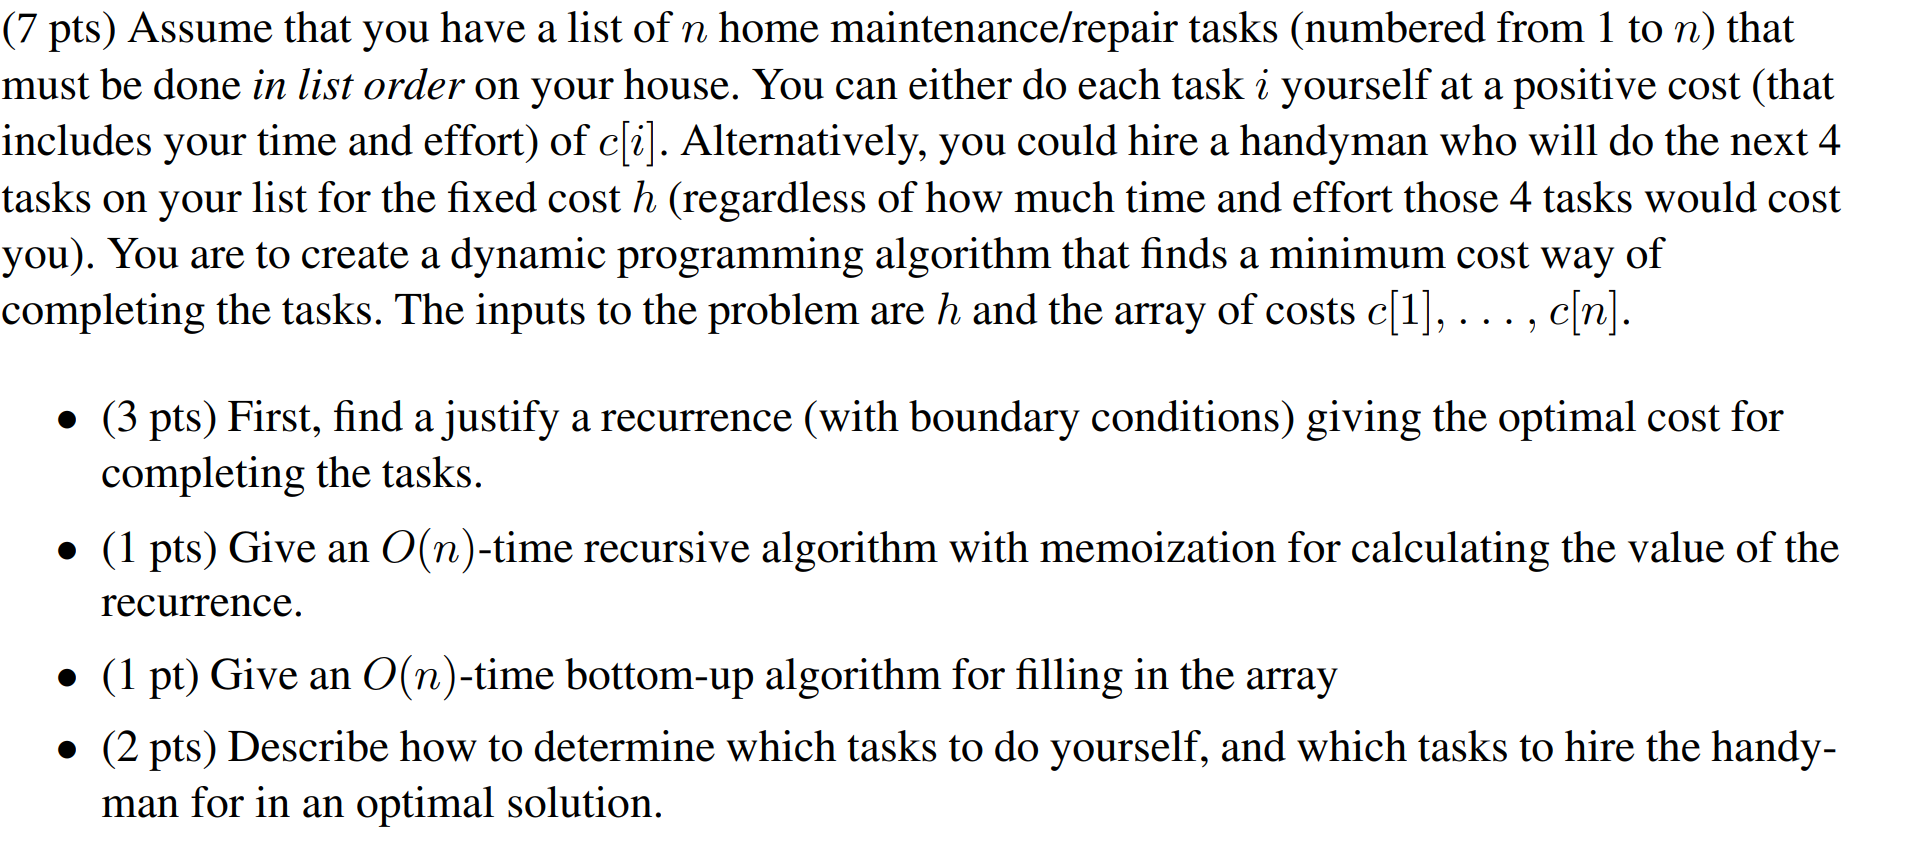
\includegraphics[scale=0.24]{4.png}
\begin{proof}[Solution for a]
	Let the optimal total cost is in array o[n]\\
	$o[i]=o[i-4]+min(h,c[i-3]+c[i-2]+c[i-1]+c[i])$\\
	If $i<4$, $o[i] = sum$(c[j: for j=0 to i]).\\
	Since $o(n)$ be the optimal solution, let $o(n-4)$ be the optimal solution for that.
\end{proof}
\begin{proof}[Solution for b]
	Set up a array o[n] to save the value during the recurrence.
	\begin{lstlisting}[language={python},numbers=left,numberstyle=\tiny,%frame=shadowbox,  
		rulesepcolor=\color{red!20!green!20!blue!20},  
		keywordstyle=\color{blue!70!black},  
		commentstyle=\color{blue!90!},  
		basicstyle=\ttfamily]  
		
o[] = int [n+1]
find(c[],n,h):
	if n<4:
		for j=0 to n:
			sum += c[j]
		o[n] = sum
	else:
		o[n] = find(c[],n-4,h)+min(h,c[n-3]+c[n-2]+c[n-1]+c[n])
	return o[n]
	\end{lstlisting}
\end{proof}
\begin{proof}[Solution for c]
	Fill the array just use the recurrence in the solution a.
	\begin{lstlisting}[language={python},numbers=left,numberstyle=\tiny,%frame=shadowbox,  
	rulesepcolor=\color{red!20!green!20!blue!20},  
	keywordstyle=\color{blue!70!black},  
	commentstyle=\color{blue!90!},  
	basicstyle=\ttfamily]  
	
	fill(c[],n):
		o[] = int [n+1]
		for i=1 to n:
			if i<4:
				o[i] = sum(c[j: for j in range(i)])
			else:
				o[i] = o[i-4]+min(h,c[i-3]+c[i-2]+c[i-1]+c[i])
		return o[n]
	\end{lstlisting}
\end{proof}
\begin{proof}[Solution for d]
	First we need an array P and initialize all element to 0 to save the result. Thinking from the task after the last element, which can be considered as "n+1" task. Using the recurrence before, then we can compare task "n", "n-1", "n-2", "n-3" with h(if $n>4$). If the first one is faster, then mark the four task to 1 in array P to represent these tasks needs to do by myself. Otherwise, stay them to 0.
\end{proof}
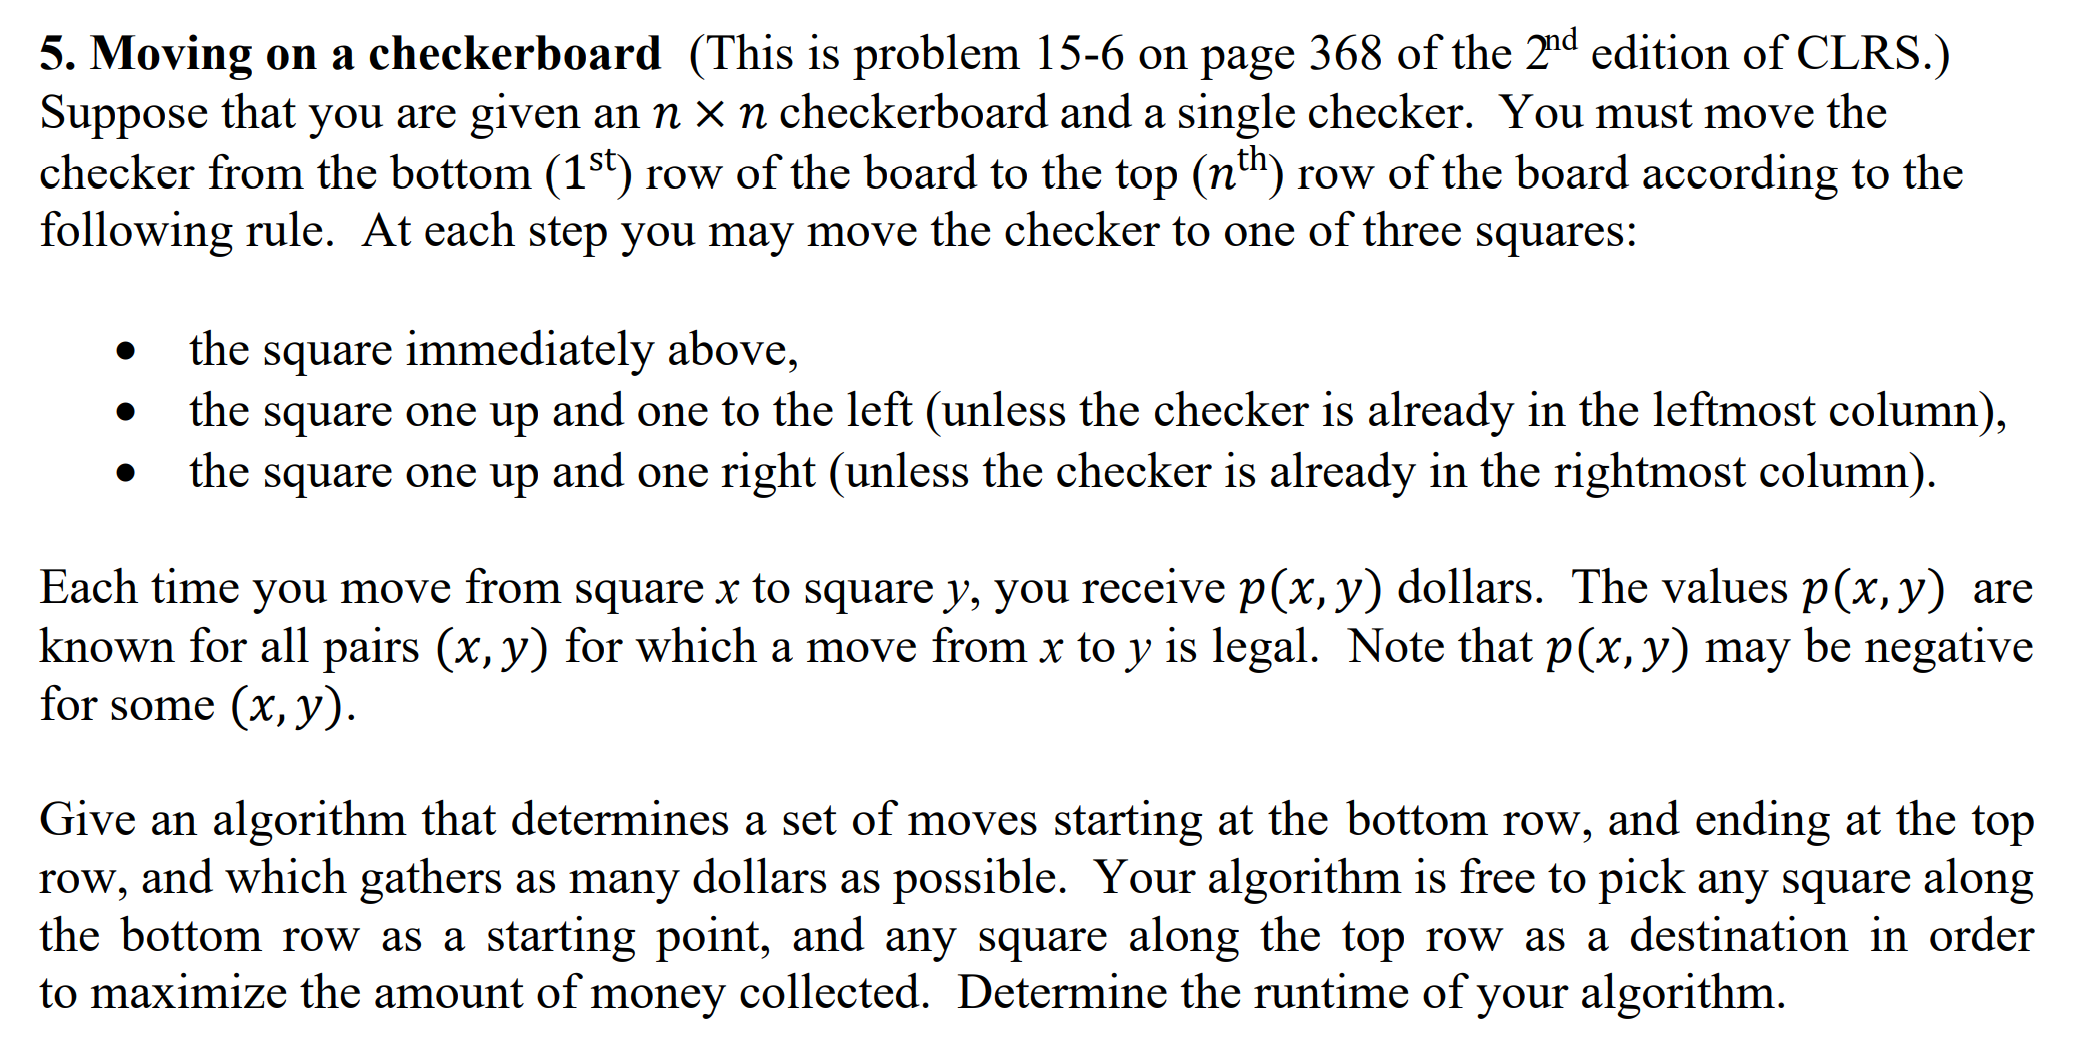
\includegraphics[scale=0.23]{5.png}
\begin{proof}[Solution]
	1. Proof of optimality
	This problem exhibits optimal substructure. We can prove by contradiction. Let q[a][n] is optimal solution for the final result, that a is the value that make the profit largest in last column, q[b][n-1] be the optimal solution for the next to last line. Assume there exist other optimal solution q[c][n-1], then we can replace q[b][n-1] with q[c][n-1] that contradicts that q[a][n] is the optimal solution, since q[a][n] is based on q[b][n-1].
	2. Recurrence
	Since no matter what, we need to move up a line. We can consider the optimal solution is saved in a 2-dimensional q[][], then the final solution is max(q[][n]) that is the largest value in the last column. The recurrence is to find the optimal solution in line below, e.g., q[n][n] = max(max[q[][n-1]]+p($dot_x$,[n][n])). x represent the dot position that make the whole equation maximum. The pseudo code to find the maximum is like this:
	\begin{lstlisting}[language={python},numbers=left,numberstyle=\tiny,%frame=shadowbox,  
		rulesepcolor=\color{red!20!green!20!blue!20},  
		keywordstyle=\color{blue!70!black},  
		commentstyle=\color{blue!90!},  
		basicstyle=\ttfamily]  
		
		len = len(p[][])
find(x,y):
	if x<1 or x>len or y<1 or y>len:
		return negative infinity # represent illegal move
	elif x=1:
		return 0
	else:
		return max(find(x-1,y-1),find(x-1,y),find(x-1,y+1))
		
	\end{lstlisting}
	3. Algorithm
	We need to first fill up the checkerboard with the optimal profit for each square, then we can find the maximum profit path. The pseudo code to find maximum is like this:
	\begin{lstlisting}[language={python},numbers=left,numberstyle=\tiny,%frame=shadowbox,  
		rulesepcolor=\color{red!20!green!20!blue!20},  
		keywordstyle=\color{blue!70!black},  
		commentstyle=\color{blue!90!},  
		basicstyle=\ttfamily]  
		#fill the checkerboard c[][]
		len = len(p[][])
fill(p[][]):
	for i=0 to len:
		for j=0 to len:
			if i = 0:
				c[i][j] = 0
			else:
				# first save the square pos
				dot_x = max(c[i+1][j-1],c[i][j-1],c[i-1][j-1])
				c[i][j] = p(dot_x, dot_[i][j]) + \
				max(c[i+1][j-1],c[i][j-1],c[i-1][j-1])
	\end{lstlisting}
	4. Sequence
	Then if we want to know the path, just save the every result in each iteration when doing $find$ in the first part.
	\begin{lstlisting}[language={python},numbers=left,numberstyle=\tiny,%frame=shadowbox,  
		rulesepcolor=\color{red!20!green!20!blue!20},  
		keywordstyle=\color{blue!70!black},  
		commentstyle=\color{blue!90!},  
		basicstyle=\ttfamily]  
		
		len = len(p[][])
		print_path(x,y):
			if c[x][y]=0:
				return
			print(x,y)
			print_path(max(c[i+1][j-1],c[i][j-1],c[i-1][j-1]))
	\end{lstlisting}
	5. Runtime
	The runtime of my algorithm is $O(n^2)$
\end{proof}



\begin{thebibliography}{ch}
\bibitem{ch} https://www.chegg.com/homework-help/questions-and-answers/2-read-coin-changing-problem-handout-dynamic-programming-solution-presented-reference-reca-q44597504
\end{thebibliography}


\end{document}
